\begin{activity} \label{A:9.2.7}

\begin{figure}[h]
\begin{center}
\begin{minipage}{3in}
\begin{center}
%\resizebox{!}{2.25in}{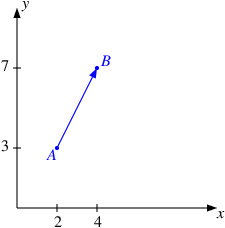
\includegraphics{figures/9_2_Vector_magnitude1}}
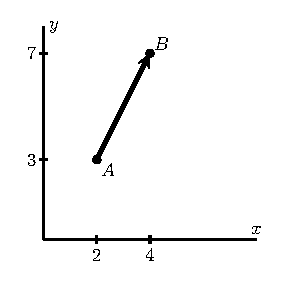
\includegraphics{figures/fig-9-20.eps}
\end{center}
\caption{The vector defined by $A$ and $B$.} %$\overrightarrow{AB}$.
\label{F:9.2.vector_magnitude}
\end{minipage}
\begin{minipage}{3in}
\begin{center}
%\resizebox{!}{2.25in}{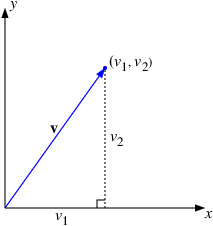
\includegraphics{figures/9_2_Vector_magnitude2}}
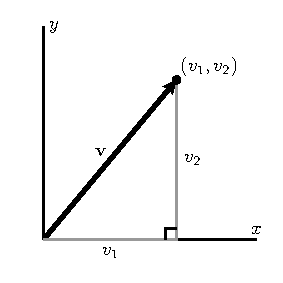
\includegraphics{figures/fig-9-21.eps}
\end{center}
\caption{An arbitrary vector, $\vv$.}
\label{F:9.2.vector_magnitude2}
\end{minipage}
\end{center}
\end{figure}
	\ba
	\item Let $A = (2,3)$ and $B = (4,7)$, as shown in Figure \ref{F:9.2.vector_magnitude}. Compute $|\overrightarrow{AB}|$.


	\item Let $\vv = \langle v_1, v_2 \rangle$ be the vector in $\R^2$ with components $v_1$ and $v_2$ as shown in Figure \ref{F:9.2.vector_magnitude2}. Use the distance formula to find a general formula for $|\vv|$.


	\item Let $\vv = \langle v_1, v_2, v_3 \rangle$ be a vector in $\R^3$. Use the distance formula to find a general formula for $|\vv|$.

        \item Suppose that $\vu = \langle 2,3\rangle$ and $\vv =
          \langle -1,2\rangle$.  Find $|\vu|$, $|\vv|$, and
          $|\vu+\vv|$.  Is it true that $|\vu + \vv| = |\vu|+|\vv|$?

        \item Under what conditions will $|\vu+\vv| = |\vu|+|\vv|$? (Hint: Think about how $\vu$, $\vv$, and $\vu+\vv$ form the sides of a triangle.)

        \item With the vector $\vu = \langle 2,3\rangle$, find the
          lengths of $2\vu$, $3\vu$, and $-2\vu$, respectively, and use proper notation to label your results.  

        \item If $t$ is any scalar, how is $|t\vu|$
          related to $|\vu|$?

        \item A {\bf unit vector} is a vector whose magnitude is 1.
          Of the vectors ${\bf i}$, ${\bf j}$, and ${\bf i} + {\bf
            j}$, which are unit vectors?

        \item Find a unit vector $\vv$ whose direction is the same as
          $\vu = \langle 2, 3\rangle$. (Hint: Consider the result of part (g).)


	\ea


\end{activity}
\begin{smallhint}

\end{smallhint}
\begin{bighint}

\end{bighint}
\begin{activitySolution}
\ba
	\item In this case we have $\overrightarrow{AB} = \langle 2,4\rangle$, so 
\[|\overrightarrow{AB}|  = \sqrt{2^2+4^2} = \sqrt{20}.\]
	\item The distance formula tells us that 
\[|\vv| = \sqrt{v_1^2 + v_2^2}.\]
	\item The distance formula tells us that 
\[|\vv| = \sqrt{v_1^2 + v_2^2+v_3^2}.\]
    \item We have $|\vu| = \sqrt{13}$, $|\vv| = \sqrt{5}$, while $|\vu+\vv| = |\langle 1,5\rangle| = \sqrt{26}$. So $|\vu + \vv| \neq |\vu|+|\vv|$.
    \item Since $\vu$, $\vv$, and $\vu+\vv$ form the sides of a triangle, and $\vu+\vv$ provides a straight path from the tail of $\vu$ to the tip of $\vv$, the length of $\vu+\vv$ should be longer that the sum of the lengths of the other sides, unless $\vu$ and $\vv$ are on the same ray. 
     \item In this case we have 
\begin{align*}
|2\vu| &= |\langle 4,6 \rangle | = \sqrt{52} \\
|3\vu| &= |\langle 6,9 \rangle | = \sqrt{117} \\
|-2\vu| &= |\langle -4,-6 \rangle | = \sqrt{52} \\
\end{align*}
    \item Note that if $\vu = \langle u_1, u_2\rangle$, then 
\[|t\vu| = |\langle tu_1, tu_2 \rangle | = \sqrt{t^2u_1^2 + t^2u_2^2} = \sqrt{t^2}\sqrt{u_1^2+u_2^2} = |t||\vu|.\]
This same argument applies in any dimension, so we conclude that 
\[|t\vu| = |t||\vu|.\]
    \item Since $|{\bf i}| = |\langle 1,0 \rangle | = 1$, $|{\bf j}| = |\langle 0,1 \rangle | = 1$, and $|{\bf i }+ {\bf j}| = |\langle 1,1 \rangle | = \sqrt{2}1$, we see that only ${\bf i}$ and ${\bf j}$ are unit vectors. 
     \item As we saw earlier, 
\[|t\vu| = |t||\vu|,\]
So 
\[\left| \frac{1}{|\vu|} \vu \right| = \frac{1}{|\vu|} |\vu| = 1.\]
Therefore, the vector $\frac{1}{13} \langle 2,3\rangle$ is a unit vector in the direction of $\vu = \langle 2, 3\rangle$.
	\ea
\end{activitySolution}
\aftera
